\question[3]
Schreibe eine Funktion \texttt{baum}, die den abgebildeten Baum zurückgibt.
Nutze dazu unsere Baum-Klasse.
Verschachtele die Baum-Aufrufe aus Lesbarkeitsgründen
höchstens einmal und gib den temporären Teilbäumen sprechende Namen.

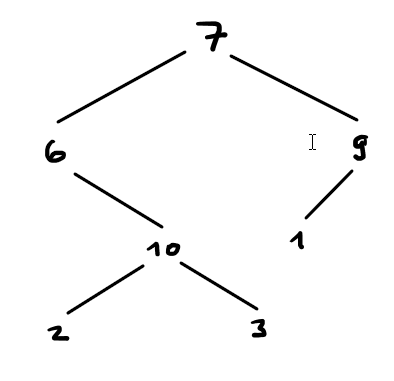
\includegraphics[height=4cm]{\pfad/Baum/Aufgaben/baumdef_01/baumdef_01.png}

\begin{solutionbox}{5cm}
\begin{lstlisting}
def baum():
    b10 = Baum(10,Baum(2),Baum(3))
    b6 = Baum(6,None,b10)
    b9 = Baum(9,Baum(1),None)
    b7 = Baum(7,b6,b9)
    return b7
\end{lstlisting}
\end{solutionbox}
